\documentclass[12pt,pdftex,titlepage]{report}

\author{\textbf{Noah Santschi-Cooney}
\\\\\\\small{Final Year Project - BSc in Computer Science}
\\\\\\\small{Jason Quinlan}
\\\\\\\small{Department of Computer Science}
\\\small{University College Cork}}
\title{\textbf{Alternative Visualisations of Distributed Tracing data in a complex, large-scale distributed system}}
\date{\vfill\small{3rd April 2020}}

\usepackage[dvipsnames]{xcolor}
\usepackage[utf8]{inputenc}
\usepackage[english]{babel}
\pagenumbering{roman}

\usepackage{graphicx}
\graphicspath{{./assets/}}

\PassOptionsToPackage{hyphens}{url}\usepackage{url}
\usepackage{microtype, caption, copyrightbox, textcomp, hyperref, listings, assets/listings-kotlin, assets/listings-graphql}
\captionsetup[lstlisting]{font={scriptsize},width=0.8\linewidth}
\captionsetup[figure]{font={scriptsize},width=0.8\linewidth}

\hypersetup{
    colorlinks,
    citecolor=black,
    filecolor=black,
    linkcolor=black,
    urlcolor=black
}
\lstset{
    frame=leftline,
    basicstyle=\scriptsize\ttfamily,
    keywordstyle=\color{Blue},
    emphstyle=\bfseries,
    numbers=left,
    numbersep=5pt,
    showstringspaces=false, 
    stringstyle=\color{ForestGreen},
    commentstyle=\color{gray},
    tabsize=4
}

\makeatletter
\def\@makechapterhead#1{%
  \vspace*{20\p@}% <----------------- Space from top of page to Chapter #
  {\parindent \z@ \raggedright \normalfont
    \ifnum \c@secnumdepth >\m@ne
        \huge\bfseries \thechapter.\ % <-- Chapter # (without "Chapter")
    \fi
    \interlinepenalty\@M
    #1\par\nobreak% <------------------ Chapter title
    \vskip 20\p@% <------------------ Space between chapter title and first paragraph
  }}
\makeatother

\begin{document}
    \maketitle    

    \chapter*{Abstract}
        \addcontentsline{toc}{chapter}{Abstract}
        Modern Internet services are often implemented as complex, large-scale distributed systems. These applications are constructed from collections 
        of software modules that could span many thousands of machines across multiple physical facilities. With the rise of modern Micro-service and 
        Service-Oriented designs, traditional tooling used to monitor application behaviour is no longer viable, especially at scale. 
        
        To understanding the flow and life cycle of a unit of work performed in multiple pieces across various components in a distributed system, the concept of 
        Distributed Tracing was born. Distributed Tracing was first introduced to the mainstream world in 2010 after the publication of Google’s Dapper
        paper. Since then, various vendors have come out with their own Dapper-inspired services, most of them based off flame or timeline graphs. 
        
        The goal of this project is dual-faceted:
        \begin{itemize}
            \item Explore and research possible alternative uses and visualisation methods utilising data collected from distributed tracing clients.
            \item Implement one or more of the proposed alternatives.
        \end{itemize}

    \chapter*{Declaration of Originality}
        \addcontentsline{toc}{chapter}{Declaration of Originality}
        In signing this declaration, you are confirming, in writing, that the submitted work
        is entirely your own original work, except where clearly attributed otherwise, and
        that it has not been submitted partly or wholly for any other educational award. I
        hereby declare that:
        \begin{itemize}
            \item this is all my own work, unless clearly indicated otherwise, with full and proper accreditation;  
            \item with respect to my own work: none of it has been submitted at any educational institution contributing in any way to an educational award;
            \item with respect to another’s work: all text, diagrams, code, or ideas, whether verbatim, paraphrased or otherwise modified or adapted, 
            have been duly attributed to the source in a scholarly manner, whether from books, papers, lecture notes or any other student’s work, whether
            published or unpublished, electronically or in print.
        \end{itemize}   
        \vspace{10mm}
        Signed: \dotfill
        \\\\
        Date: \dotfill

    \chapter*{Acknowledgements}
        \addcontentsline{toc}{chapter}{Acknowledgements}
        
    \tableofcontents

    \chapter{Introduction}
    \pagenumbering{arabic}
    \setcounter{page}{1}
        \section{Problem}
            Within the last decade, the way modern applications are being built and deployed has changed dramatically. With the shift from collocation to cloud computing,
            virtual machines to containerization technologies, monoliths to micro-services and beyond, software developers have been able to adjust to 
            the monotonical increase in internet traffic, shipping highly scalable, efficient and reliable software that meets the ever-demanding needs of their customers
            with the slew of emerging technologies.

            While this shift has undoubtedly solved many issues with regards to scaling services in terms of both maintainability as feature sets increase and in keeping up
            with an every larger number of online users, it has introduced a whole new suite of problems that needed to be addressed in terms of reliability and application 
            monitoring. With the splitting of monolithic applications into micro-services, the failure points are extended to issues in the network, including but not limited
            to network congestion, DNS resolution errors etc. Developers are ever more inclined to code failure resilience into their applications, falling back gracefully in 
            apprehension of unforeseeable failures.

            As these new distributed system architectures evolved and became ever more widespread, traditional application monitoring tools consistently fell short of providing
            developers and systems operators with the means to gain introspection into systems and their failures in production scenarios. Traditional monolithic systems often
            utilized logging and metrics to gain introspection into the application and for alerting on rules respectively. For such systems, these process-scoped measures often 
            provided good insight into a system, correlating logs on their thread identifier/name as each thread would handle a single request sequentially. As these systems 
            adopted asynchronous execution models, where a request's lifetime may not be confined to a single thread, the previous approach no longer works, making observing
            the behaviour of such systems very difficult unless developers annotated logs with request-scoped identifiers. The final evolution of concurrency in application systems is
            commonly referred to as \textit{distributed concurrency}. This is often associated with micro-services, in which a request is no longer constrained to being executed
            in a single process, but may span multiple processes and even servers. Figure~\ref{fig:concurrency} highlights this evolution, from simple, single threaded applications,
            through to micro-service-like architectures.

            \begin{figure}[htb!]
                \centering
                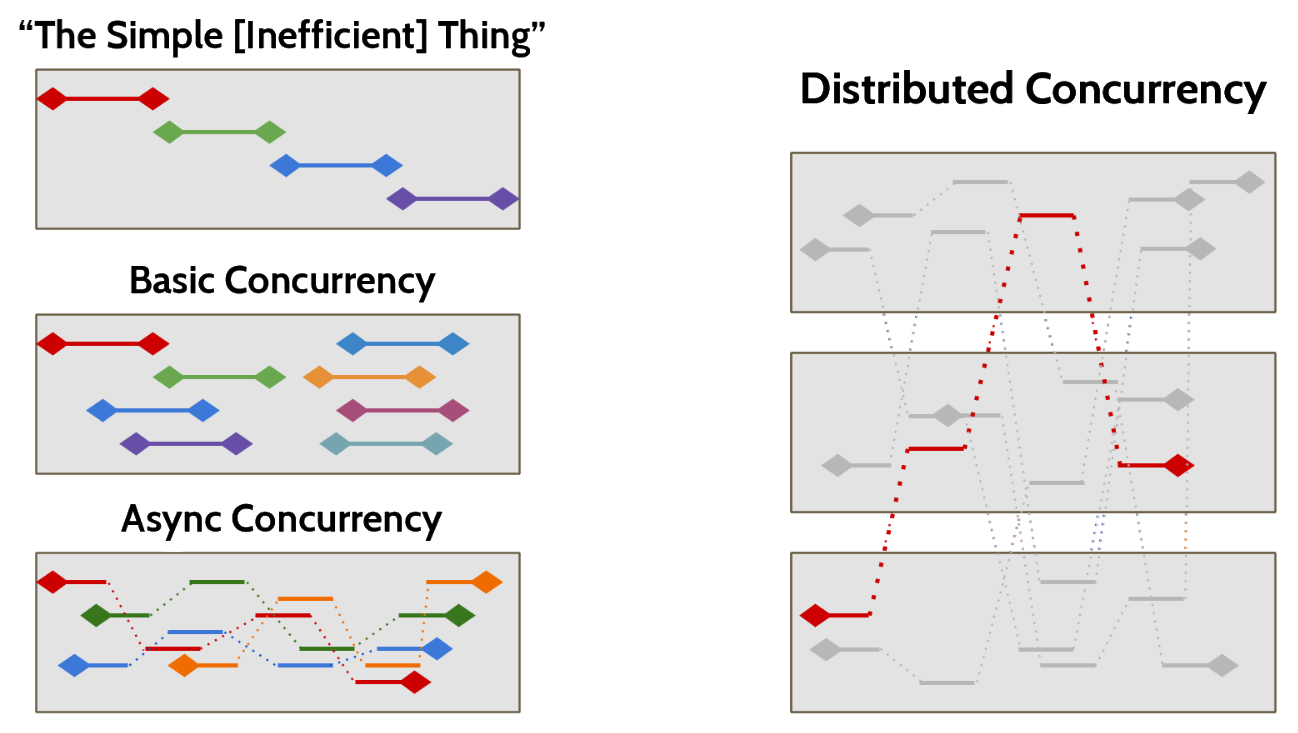
\includegraphics{concurrency.png}
                \caption{Evolution of concurrent systems.}
                \label{fig:concurrency}
            \end{figure}
        
        \section{Debuggers}
            In traditional single process applications, debugger tools, both standalone and bundled with integrated development environments (IDEs), are invaluable in their
            use of isolating bugs in codebases of any size. They have the capability to give complete overview of stack and heap allocated variables as well as being able to set
            breakpoints to step through code. Figure~\ref{fig:debugger} highlights the various insights and utilities provided by such tools, including the display of call stacks,
            local and global variables as well as various utilities to step through code at the line and function levels.

            \begin{figure}[hbt!]
                \centering
                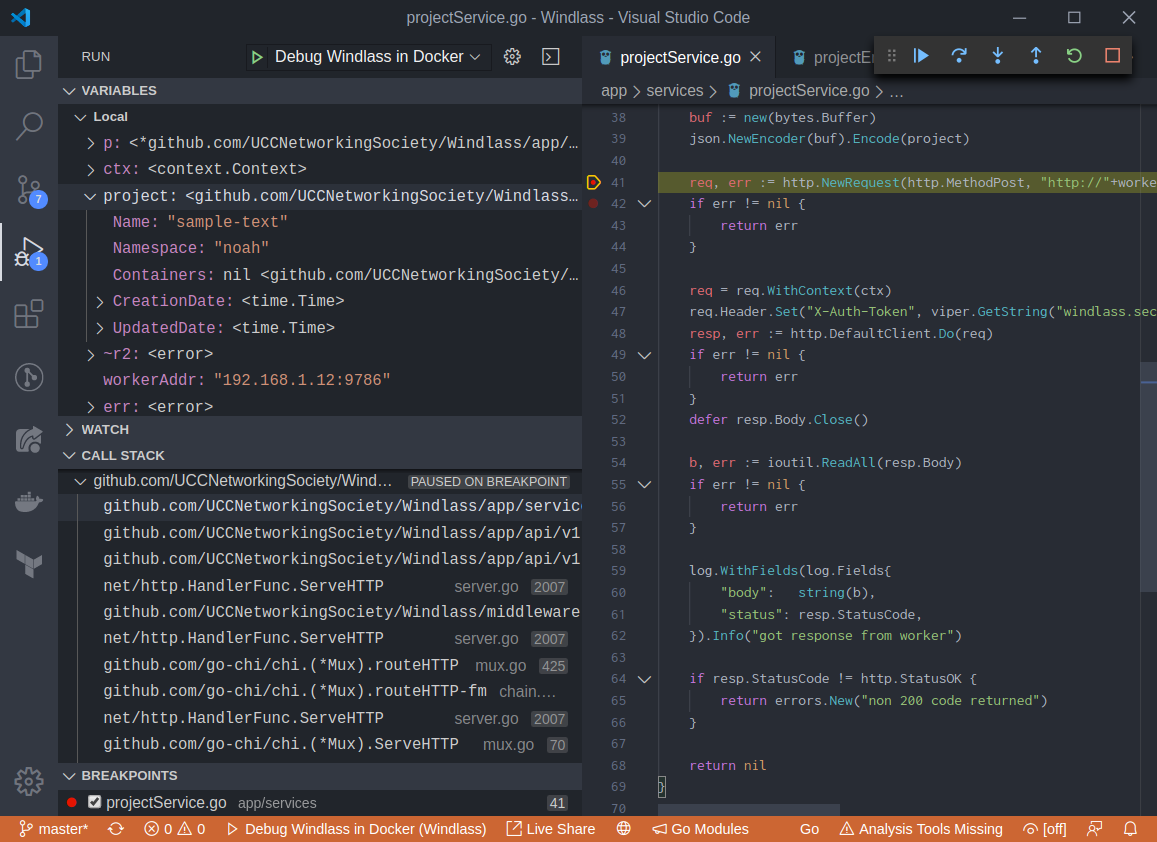
\includegraphics[scale=0.335]{debugger}
                \caption{Screenshot of the Visual Studio Code debugger in action. Clockwise, shown are an expandable list of local and global variables, the currently open file view
                with the line currently halted on highlighted along with controls for stepping and finally the function call stack.}
                \label{fig:debugger}
            \end{figure}
            
            However, it is often infeasible to use them in production scenarios due to their nature of halting complete execution of the process.
            This makes it unsuitable for debugging issues that manifest in production that developers are finding it difficult to reproduce in development scenarios, as is often
            a common scenario due to subtle parity differences between development and production systems.

        \section{Distributed Tracing}
            As traditional tooling is not designed to accommodate for this distributed concurrency system, new methodologies were needed to regain observability into the systems.
            Observing single systems individually, as was done with traditional tooling, no longer painted the full picture of a request as it travels through multiple system 
            components. Distributed tracing systems and platforms build upon the concepts of reconstructing a request from a series of event streams from each component involved
            in the request, with distributed context propagation and aggregation, building causality graphs from a request-centric point of view.

            \begin{figure}[hbt!]
                \centering
                \copyrightbox[r]{
                    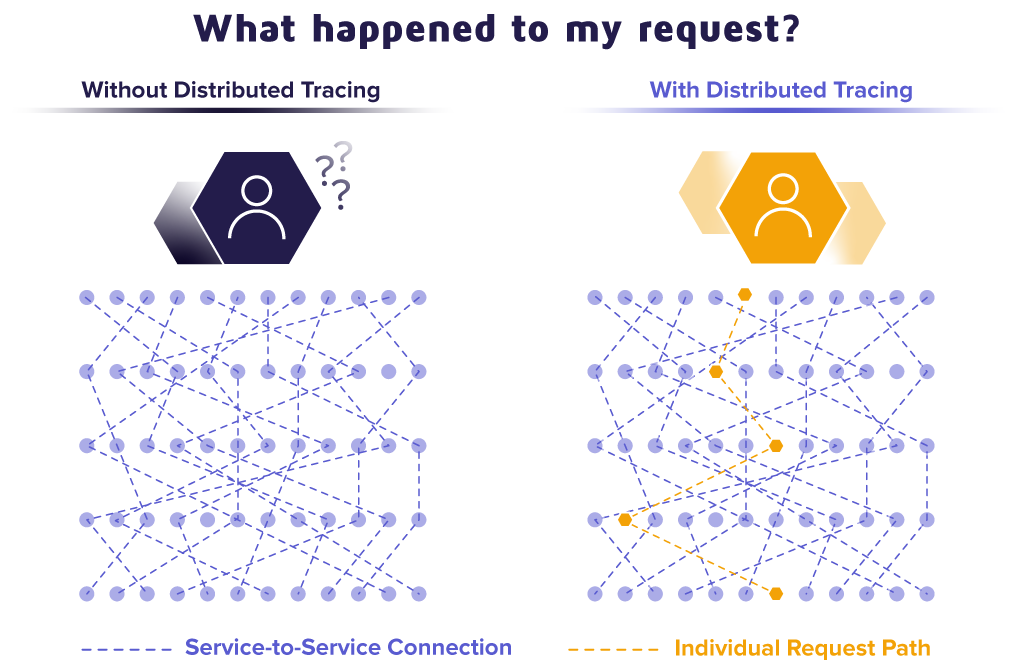
\includegraphics[scale=1.7]{distributed}
                }{
                    \tiny{\textcopyright Nic Munroe "Hit the Ground Running with Distributed Tracing Core Concepts" on Medium}
                }
                \caption{Depiction of a complex distributed system with much inter-connectivity between services.}
                \label{fig:dist}
            \end{figure}

            Code is instrumented at various points of interest, recording annotated events with metadata such as the user ID associated with the request, SQL statements being 
            executed on a database etc. These events are often shipped to a collector/exporter, from which they are either stored in a database or sent to a hosted vendor, such as
            LightStep or Honeycomb, after which they can be queried, retrieved and displayed.

        \section{Motivation \& Goals}
            As distributed tracing is still a relatively new idea and only as of recently gathering mainstream interest in the industry, research and advancements on the topic are 
            as of yet still sparse. Current vendors often provide a limit set of capabilities and operations that can be performed on the data output from instrumented distributed systems,
            most commonly simple expandable \textit{gantt charts} or, less commonly, simple, mostly static, service dependency graphs that offer little value and utility.

            To further research in this field, the project will attempt to explore alternative and hopefully improved ways of consuming and presenting the data from instrumented
            applications. Two ideas were planned to be explored and, if possible, implemented as proof of concepts:

            \begin{itemize}
                \item Advancements in Service Topology/Dependency graphs
                \item Editor Debugger integration                
            \end{itemize}

            % TODO:
            The viability and findings of both explored options will be discussed, with performance benchmarks where relevant being presented to highlight the feasibility of different
            approaches 

        \section{Project Summary}
            This project builds upon the concepts of distributed tracing, exploring ways to provide novel and high-value derivable ways of visualizing and presenting distributed tracing
            data to developers. Modern standards, tools and integrations will be utilized to test the viability of less common and unexplored visualizations of distributed tracing data.

            In Chapter 2, the history of distributed tracing will be introduced, while also covering some common vocabulary relevant to the topic and where they originated. It will also
            cover some of the standards that this project builds around. In Chapter 3, the project architecture design choices will be discussed and how they impacted the project, ranging
            from the frontend frameworks chosen to the backend API and supporting services that power the various implementations. Finally, the different visualizations will be evaluated
            on the value the provide as well as the feasibility of utilizing them in real-world scenarios. Chapters 5 and 6 will draw the writeup to a conclusion, detailing the closing
            thoughts and putting forward ideas for future work on the ideas explored in this project.

    \chapter{Background}
        \section{History}
            \subsection{Dapper}
                Released in April 2010, Google published a paper describing the design decisions behind an in-house implementation 
                of distributed tracing, named Dapper. It is commonly believed that this paper describes the common ancestor to 
                many tools that implement a form of distributed tracing.

                The Dapper paper introduces some of the core primitives that underpin modern day standards. Most notable are the concepts
                of a directed acyclic graph (DAG) called a \textit{trace tree} and its nodes, which are referred to as \textit{spans}. 
                The trace tree forms a relationship between spans, not unakin to a tree of stack frames that may be generated by
                gathering stack frames over time, albeit generally at a much higher level than at the level of individual subroutine calls. 

                Figure~\ref{fig:dappertrace} illustrates a trace tree with five spans. Each span is shown to contain 3 specific pieces of
                metadata alongside the start and end timestamps necessarily to reconstruct the temporal relationships: a human-readable
                \textit{span name}, an integer \textit{span ID} and an integer \textit{parent ID}. The latter two
                data points are used to reconstruct the relationship between individual spans. A span without a parent ID becomes the 
                \textit{root span} of a trace tree. Not shown is another important but, as of right now, not relevant piece of metadata, the 
                \textit{trace ID}, which is common amongst all spans within a single trace tree.

                \begin{figure}[htb!]
                    \centering
                    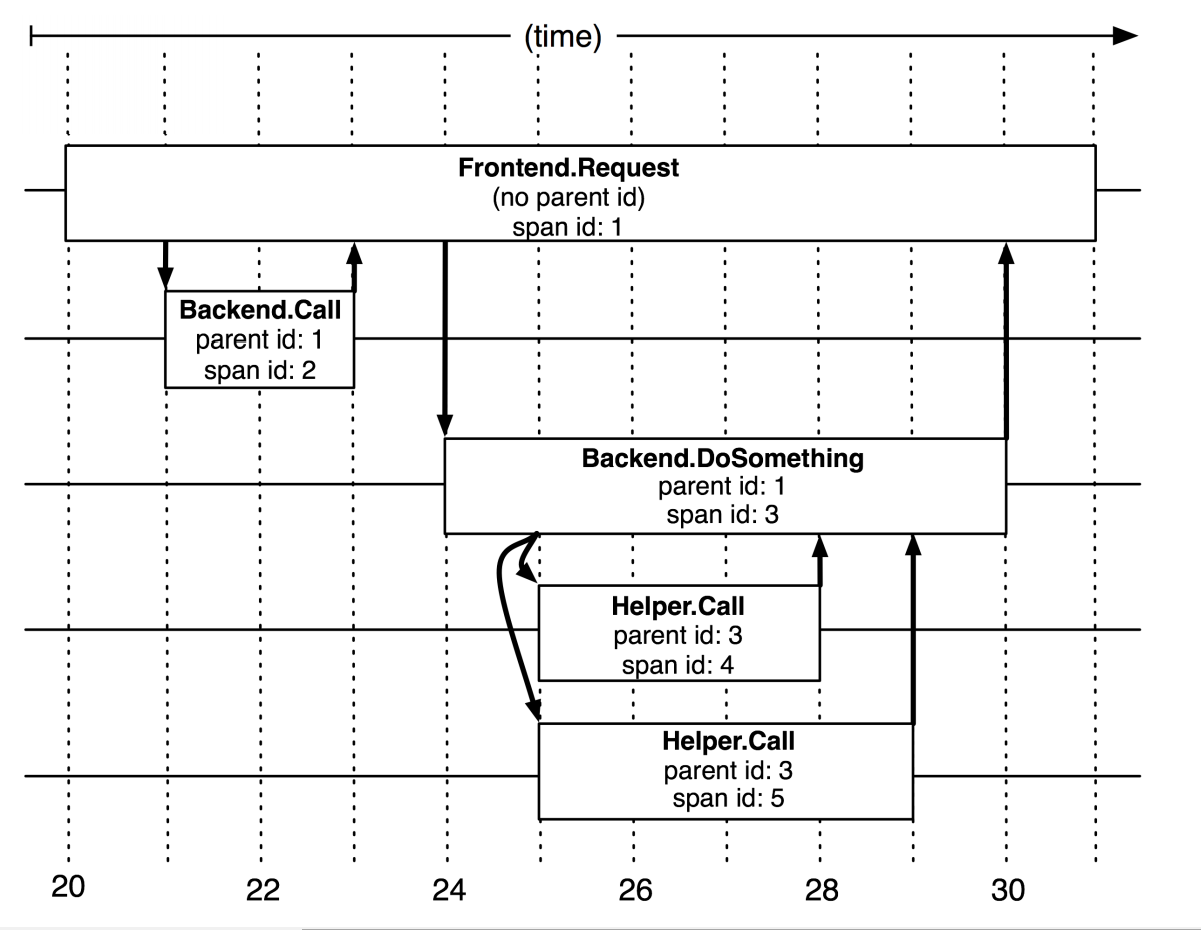
\includegraphics[scale=1]{dappertrace}
                    \caption{The relationships between traces in a trace tree.}
                    \label{fig:dappertrace}
                \end{figure}

                As described thus far, Dapper trace trees allow for a detailed view of the relationships of distributed systems within
                Google. When using this data for debugging or performance analysis, it can often be convenient or even necessary to 
                have additional context surrounding a trace tree or its individual spans. As such, the paper describes a simple API 
                through which application developers can provide a combination of two types of annotations: timestamped textual annotations
                and key-value, allowing for defining arbitrary equivalence classes between traces which can be operated upon in the analysis
                tools.

            \subsection{OpenTracing}
                OpenTracing\cite{opentracing} project's inception came about in October 2015, it has since become a project under the 
                Cloud Native Computing Foundation in 2016, created to standardize a set of vendor neutral and programming language agnostic
                application programming interfaces (APIs) for instrumenting code for distributed tracing. Heavily inspired by the Dapper
                paper, it borrows many of the nouns and verbs outlined in the Dapper paper, including \textit{traces} and \textit{spans}.
                Dapper's timestamped annotations are referred to as \textit{logs} in the OpenTracing specification, while the key-value pairs
                are named \textit{tags}. 

                The OpenTracing API also specifies how a trace cross process boundaries, so that spans created in different processes can be
                associated with a common trace tree. This was named the \textit{span context} and at its most basic level contains the 
                overlying trace ID as well as the current span ID. With this, new spans generated across process boundaries have the ability to
                to specify their parent span as well as their common trace, without propagating an entire span, which may prove costly as more
                tags and logs are attached to a span.

                Figure~\ref{fig:opentracing} shows a timeline based visualization of where the different components of the OpenTracing API interface are utilized in
                the larger picture of creating a span through use of distributed context propagation in the span context construct to build the span tree across
                process and network boundaries.
                
                \begin{figure}[hbt!]
                    \centering
                    \copyrightbox[r]{
                        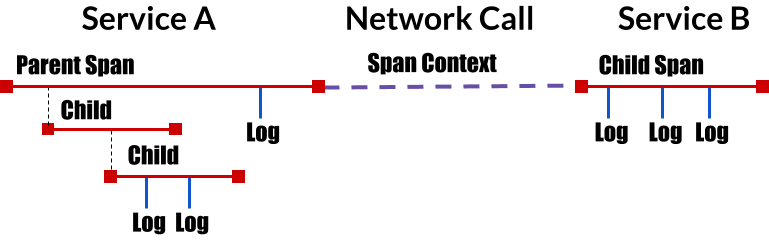
\includegraphics[scale=0.5]{opentracing}
                    }{\tiny{\textcopyright OpenTracing "OpenTracing Overview"}}
                    \caption{Infographic visualizing the different components that make up the OpenTracing API interface and how they relate to different services
                    and the network}
                    \label{fig:opentracing}
                \end{figure}

                As there are multiple output sinks which can consume OpenTracing data, from self hosting services such as Jaeger to hosted vendors like LightStep, and given that
                different platforms may have different, vendor-specific options for operations such as access control, authorization etc, vendors provide different mechanisms
                and attributes for creating instances of OpenTracing API \textit{tracers} implementations.

                \begin{lstlisting}[caption=Example Golang snippet of instatiating a Datadog OpenTracing compatible tracer., language=Go, gobble=20]
                    package main

                    import (
                        "gopkg.in/DataDog/dd-trace-go.v1/ddtrace"
                        "gopkg.in/DataDog/dd-trace-go.v1/ddtrace/opentracer"
                        "github.com/opentracing/opentracing-go"
                    )

                    // Start a Datadog tracer, optionally providing a set of options,
                    // returning an opentracing.Tracer which wraps it.
                    t := opentracer.New(
                        tracer.WithAgentAddr("host:port"),
                        tracer.WithServiceName("sample-text"))

                        // Use it with the OpenTracing API, setting it as global.
                    opentracing.SetGlobalTracer(t)
                \end{lstlisting}

                \newpage
                \begin{lstlisting}[caption=Example Golang snippet of instatiating a Jaeger OpenTracing compatible tracer., language=Go, gobble=20]
                    package main

                    import (
                        "github.com/uber/jaeger-client-go"
                        "github.com/uber/jaeger-client-go/transport"
                        "github.com/opentracing/opentracing-go"
                    )

                    // Start a Jaeger tracer, supplying the sampling strategy and the
                    // reporter configuration.
                    t, closer := jaeger.NewTracer(
                        "sample-text",
                        jaeger.NewConstSampler(true),
                        jaeger.NewRemoteReporter(transport.NewHTTPTransport("host:port")))
                    defer closer.Close()

                    // Use it with the OpenTracing API, setting it as global.
                    opentracing.SetGlobalTracer(t)                    
                \end{lstlisting}

            \subsection{OpenTelemetry}
                The OpenTelemetry\cite{opentelemetry} project came about as a result of the merging of two previous projects, namely the previously mentioned OpenTracing
                project as well as OpenCensus project. The OpenCensus project originated from Google and had many similar goals to OpenTracing. Alongside having an interface
                for distributed tracing gathering, it also supported instrumenting applications to output application metrics data. To reduce the fragmentation in having
                two independent APIs for distributed tracing, the two projects decided to merge into one standard going forward. At the time of writing, support for OpenTelemetry
                is still very sparse, due to the fact that it is still a very new specification set, while still being largely backwards compatible with both OpenTracing and 
                OpenCensus, providing API bridges to maintain compatibility. 

                The OpenTelemetry API improves upon OpenTracing by introducing a set specification for context propagating header keys used to identify specific values, created
                as a W3C specification. In OpenTracing API implementations, different vendors would use different keys to denote values such as the trace ID etc in, for example, 
                HTTP headers. This would break the context chain if different codebases used different vendor implementations in a service dependency graph. By demoting vendor
                libraries to providing simple \textit{exporters} that define how distributed tracing data is exported to backend systems rather than having them provide
                tracer implementations like the way it was done with the OpenTracing API, the OpenTelemetry project achieves a better level of interoperability between codebases, 
                where the OpenTelemetry \textit{collector} can act as the common sink for the different services, becoming the source of truth regarding the eventual backend system
                to which the distributed tracing data will be exported to.

                \begin{figure}[hbt!]
                    \centering
                    \copyrightbox[r]{
                        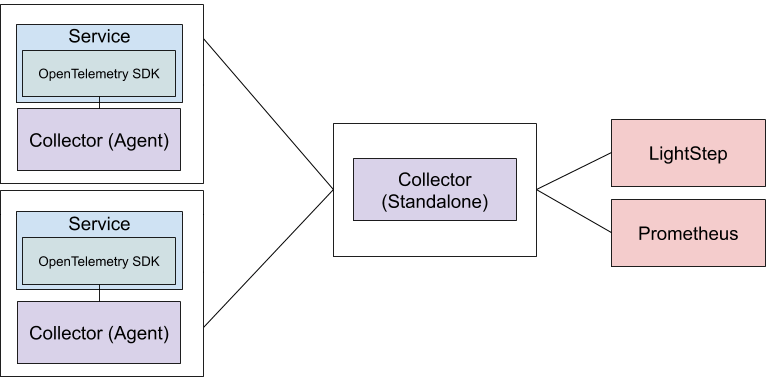
\includegraphics[scale=0.5]{opentelemetry-exporter}
                    }{\tiny{\textcopyright{LightStep "OpenTelemetry 101: What is an Exporter?"}}}
                    \caption{A high level overview of a typical OpenTelemetry setup, with services hooking into the OpenTelemetry SDK to output telemetry to
                    OpenTelemetry Collectors, which themselves forward data to the standalone Collector sink, which is configured to send metrics to a \textit{Prometheus}
                    server and distributed tracing data to the LightStep API.}
                    \label{fig:otexporter}
                \end{figure}
                

    \chapter{Design \& Implementation}
        \small{In this section, the different technical aspects will be covered, design decisions and components that played a role throughout the projects lifecycle.
        This will include third party services and the roles they played.}

        \section{Architecture Design}
            \subsection{Distributed Tracing API}
                The OpenTracing API interface was chosen as the foundation for this project. This decision was made due to the large language support and comprehensive open
                source tooling built around the OpenTracing API. It is also widely supported by many third party vendors, including LightStep, DataDog and Honeycomb amongst 
                numerous others.

                OpenTelemetry was initially considered as an alternative choice instead of OpenTracing, but was ultimately decided against due to it still being a very new
                standard, with OpenTracing having much more comprehensive support and documentation resources from both application libraries and distributed tracing tools.
                This lowered the productivity barrier, as the OpenTelemetry backing components, including the collector, introduce more complexity than what exists in a simple
                development-oriented OpenTracing setup.

                Potential explorations around the OpenTelemetry API are discussed in the \textit{Future Work} section.

            \subsection{Supporting Services}
                As both explored ideas will be interacting with distributed tracing data, there are two pieces to the puzzle of having a set of traces to work with.
                Firstly, a way of collecting trace data from applications is needed, and secondly, the database into which the data is persisted.
                
                The OpenTracing platform, Jaeger, was chosen for this project. Jaeger is wholly self-hostable, providing a convenient setup for single-machine development purposes with
                a single, all-inclusive binary available from the distribution archives, as well as a pre-built \textit{Docker} image published to DockerHub. The full Jaeger package,
                available in whole in the aforementioned all-inclusive formats, includes the trace collector, trace search and visualization user interface and agent.

                By default, the all-in-one Jaeger distribution stores all trace data in-memory. For convenience to persist data in between machine reboots, the JSON document search engine
                database, \textit{Elasticsearch}, was chosen as the storage backend for Jaeger, as one of two possible choices alongside \textit{Apache Cassandra}, a column store document
                database. The Backend API, discussed later in this chapter, interfaces with the Elasticsearch database as the source of truth for the trace data. A complementary user interface
                for Elasticsearch, maintained by the developers of Elasticsearch, \textit{Kibana}, was used throughout the development of the project to view the raw trace data as it is 
                represented in the database.

                %In line with how the OpenTracing API works with regards to tracer implementations, the Jaeger language-specific instrumenting libraries must be used to inject the Jaeger 
                %tracer implementation into the applications. A small number of 


            \subsection{Backend API}
                To query for and transform the distributed tracing data stored in Elasticsearch, an HTTP API was developed for the two codebases of the ideas explored to interface with.
                Written in Kotlin, a programming language that runs on the Java Virtual Machine, it provides a GraphQL interface to fetch the trace data from Elasticsearch. It was 
                decided that Kotlin would be the language used for the backend after evaluating the different Elasticsearch and GraphQL libraries available, of which there were libraries 
                that utilized the Kotlin \textit{Domain Specific Language} (DSL) to define the queries and schemas respectively.
                
                \subsubsection{GraphQL}
                    As an alternative to traditional RESTful HTTP services, GraphQL is both a query language and a server-side runtime for executing queries against a defined data schema
                    laid out by the type system. The type system can be shared between both servers and clients alike, allowing for a common, known data schema. The data schema consists of 
                    user defined object types representing the data, as well as two special types: the \textit{Query} type and the \textit{Mutation} type. These define the entrypoints into
                    the GraphQL server, allowing for the fetching and modification of data, and can take a defined set of arguments as defined in the schema, which may be defined as being
                    optional.\newpage

                    \begin{lstlisting}[caption={The base GraphQL schema, defining a query and data types for the trace data.}, language=GraphQL, gobble=24]
                        type Query {
                            findTrace(traceID: String): Trace
                        }

                        type Trace {
                            traceID: String!
                            spans: [Span!]!
                        }

                        type Span {
                            traceID: String!
                            spanID: String!
                            parentSpanID: String
                            duration: Int!
                            startTime: Int!
                            operationName: String!
                            serviceName: String!
                            logs: [LogPoint!]
                            tags: [Tag!]
                        }

                        type LogPoint {
                            timestamp: Int!
                            fields: [LogPointField!]!
                        }

                        type LogPointField {
                            key: String!
                            type: String!
                            value: String!
                        }

                        type Tag {
                            key: String!
                            type: String!
                            value: String!
                        }
                    \end{lstlisting}
                    
                    One of GraphQLs improvements over traditional REST is the ability to specify fields to \textit{resolve} in the server-side runtime engine. Besides preventing
                    under- and over-fetching, this also allows for the ability to selectively augment the returned data, adding extra fields or even changing existing ones on-demand,
                    all within the same query while not incurring the costs for clients that do not request them. Listing~\ref{lst:graphTrace} shows an example of selective field
                    resolving. The second query also requests the \texttt{spans} field, which could have a range of effects on the server e.g. performing an extra SQL \texttt{JOIN}
                    statement, while also resulting in potentially more data being sent down the wire.

                    \newpage
                    \begin{lstlisting}[caption={A GraphQL query to fetch a trace object and the span ID of each of its spans compared to a query to fetch the trace object, its spans and every
                        tag of every span.}, label={lst:graphTrace}, language=GraphQL, gobble=24]
                        {
                            query findTrace(traceID: "asdf") {
                                traceID
                                spans {
                                    spanID
                                }
                            }
                        }

                        {
                            query findTrace(traceID: "asdf") {
                                traceID
                                spans {
                                    spanID
                                    tags {
                                        key
                                        type
                                        value
                                    }
                                }
                            }
                        }
                    \end{lstlisting}

                \subsubsection{Interfacing with the Database}
                    As the decision was made to use the Jaeger tracing platform backed by Elasticsearch for this project, the backend server must interface with Elasticsearch
                    to be able to serve the data to the API clients that make up this project. Under these circumstances, this project could be potentially used in production
                    by teams that host a Jaeger tracing platform on their infrastructure with Elasticsearch. The backend must simply support connecting to the database, building 
                    JSON queries at either an abstracted or low level and finally being able to execute those queries against the database. Elasticsearch has first-party libraries
                    for a  large number of languages, and given Kotlin's interoperability with Java, the backend makes use of the Java Elasticsearch client library. Adding support 
                    for Apache Cassandra database would be trivial, however outside of the scope of this project.

                    While the Jaeger tracing platform is commonly employed by development teams, vendor hosted distributed tracing systems also have seen large adoption due to the 
                    fact that it allows teams to not worry about maintaining an instance of Jaeger in their infrastructure, either due to convenience, monetary costs needed to host
                    the Jaeger platform or having to maintain extra services. These vendors often do not provide a public API for querying and fetching trace data. Discussion around
                    possible solutions for these scenarios can be found in the future works section. The rest of this report works under the assumption of the Jaeger tracing platform
                    being employed, either as the sole distributed tracing system or complementary to a vendor hosted solution. 

            \subsection{Debug Adapter}
                For this part of the project, it was decided to develop the idea of integrating the telemetry from instrumented applications into the debugger API of Visual Studio Code.
                Visual Studio Code was chosen as the editor for which the integration would be built due to its extensive extensibility and first class Debug Adapter Protocol support. 
                Built in Typescript, a Javascript superset with type annotations, the service implements the Debug Adapter Protocol to bridge between the trace data stored in Elasticsearch
                and the editor to provide many of the same features one would expect from traditional debugger tools such as the GNU Project Debugger (GDB).

                Figure~\ref{fig:debug-arch} displays the general architecture of how editors and tools utilize the programs that implement the Debug Adapter Protocol to interact with
                lower level debug runtimes, such as GDB etc. Each editor or tool would contain a small, lightweight shim, one per debug adapter, that launches the debug adapter with the
                appropriate configuration, potentially with user supplied configuration data, before handing off to the in-editor/tool generic debugger that interacts with the now running
                debug adapter through the Debug Adapter Protocol.

                The Debug Adapter for this part of the project combines combines the three necessary parts in the one codebase, the shim, debug adapter and debugger runtime, for convenience
                in developing the proof of concept. It builds off the Visual Studio Code mock debug adapter, a sample codebase implementing the shim, debug adapter and a dummy debugger
                runtime in one. Heavily inspired by asynchronous event-based programming as is commonplace in the NodeJS ecosystem, the debug adapter invokes asynchronous methods on the 
                debugger runtime when it receives requests from the editor or tool in the Debug Adapter Protocol format, upon which the debugger runtime may emit events that the debug adapter
                translates into Debug Adapter Protocol events for the editor or tool to consume.

                \begin{figure}[hbt!]
                    \centering
                    \copyrightbox[r]{
                        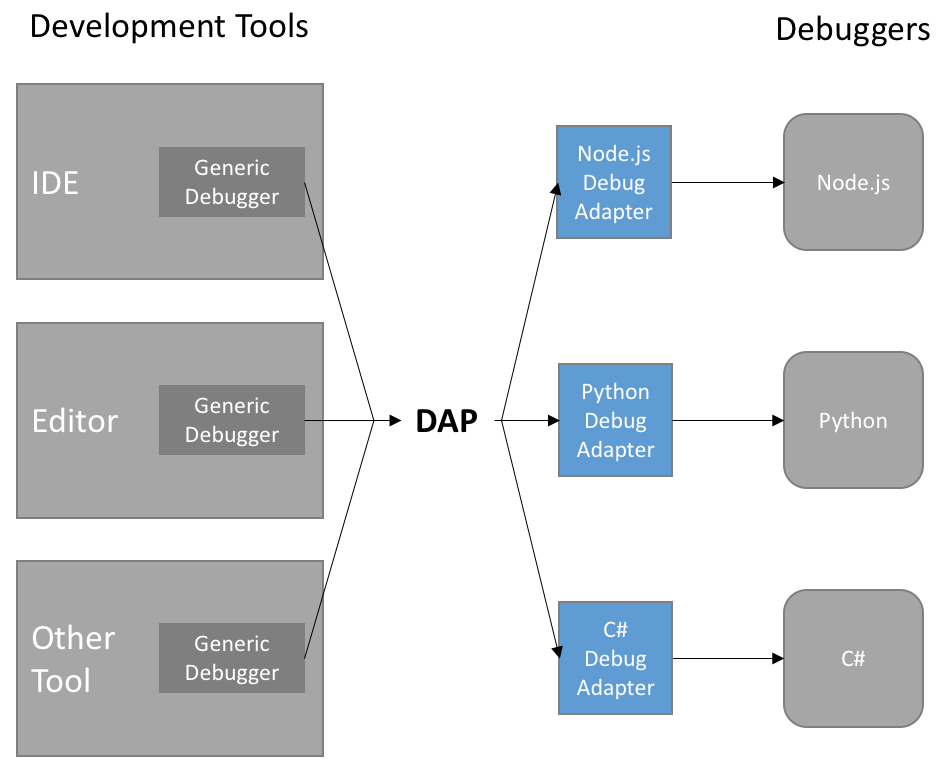
\includegraphics[scale=0.4]{debug-arch}
                    }{\tiny{\textcopyright{Microsoft Corporation. https://vscode.readthedocs.io/en/latest/extensions/example-debuggers/}}}
                    \caption{Diagram displaying the relationship between Editors and Tools, the Debug Adapter Protocol, Debug Adapters and the possible Debug Runtimes. Not shown are the
                        editor/tool dependent shims. Each \textit{Development Tool} contains a debugging utility that speaks the Debug Adapter Protocol to communicate with various Debug
                        Adapters.}
                    \label{fig:debug-arch}
                \end{figure}

                Conceptually, the role of the debug adapter created for this project is simple: given a trace ID, it should fetch the spans and their metadata for the trace ID, load the 
                source code files for each span and allow the user to step through the code on a span-by-span basis (or more granular). If successful, the user would be able to see the
                source code file and line in which the current span was started and step back and forth between spans and their respective source code files and lines. Given the focus
                around non-monorepo codebases, it should also have the ability to jump to and from files outside the currently opened codebase, assuming that the codebases for the other 
                services also reside on the user's machine.
                
                The main approach to making this set of requirements possible is by utilizing the tag constructs defined in the OpenTracing specification to carry additional runtime or
                compile time information that provides enough information to the debugger runtime. This can be done by implementing shims that wrap OpenTracing trace implementations with
                methods that add the required information as tags to newly created span instances. When the debugger runtime queries the backend API, it can request an additional field on
                the span types that the backend GraphQL resolver resolves by transforming the information gathered by the shims into a format more useful to the debugger runtime than the
                raw collected information. This results in being able to interface with the same GraphQL query as the project idea that follows this part, while not incurring the 
                transformation costs in the following idea.
                % TODO: word this better

                In practice, there are a number of challenges that arise in various parts of this concept; gathering the information required to pinpoint the source file and line varies 
                in format across different programming languages, amount of stack trace information that is to be or that can be gathered and its formats across different programming 
                languages, mapping different services to the location in the filesystem of their codebase as well as handling spans emitted from services not appropriately instrumented 
                for this to work. There are different trade-offs with various approaches to these problems that will be outlined.

                When dealing with collecting information on the source file and line number at which a span was started, there are two main approaches with highly contrasting pros and cons.
                The first approach is to simply query the runtime, where applicable, for the file path and line number associated with the function that invoked the span creation. This is often
                a relatively cheap operation, with a small footprint in the amount of data that a span is tagged with. The main downside of this approach is that while it results in a small 
                amount of extra data attached to a span, this reduced amount of information reduces the capabilities of the debugger runtime. With this information, the debugger runtime is
                limited to jumping between those single, individual points in the code at which the spans are created (this could be expanded to also wrap the log-point calls to do the same).
                
                The second approach involves querying the runtime for an entire stacktrace leading up to this point. With this approach, there is considerably more data, with all the function
                calls of the stack frame tree branch leading up to the span creation being gathered, allowing for the possibility to step back and forth at the function level rather than simply
                at the span level. In both these instances, the data is attached to spans as tags. This approach was chosen to be explored for the project due to the larger potential that accompanies
                the greater amount of data. For further processing outlined in the following paragraph, the programming language from which the span originates is added as a tag to the span.
                There are a few downsides to this approach and possible workarounds that will also be discussed.
                
                In many language implementations of the Jaeger tracer, tag values are limited in length to either 256 or 1024 characters. When dealing with stacktraces, this limit is too 
                restrictive for storing entire stacktraces. This is due to an outstanding issue in Jaeger client implementations when using UDP as the transport protocol, as span sizes
                would exceed the maximum UDP packet size of 65535 bytes\cite{udptagsize}. This makes using HTTP as the span transport method a hard requirement to avoid UDP packets being
                dropped, causing entire spans to be lost. The client implementations also provide an interface for changing the max tag value length, which must be utilised to prevent the truncating
                of the stacktraces. As this number cannot be set on a per-span basis, it must be set at a reasonably large number ahead of time based on previous examples of possible stacktrace sizes
                or the maximum value of an integer for the given platform. Another downside to full stacktraces is that the procedure for getting an entire stacktrace and transforming them can often 
                be considerably more expensive than adding simple tags to a span. Unfortunately, sampling rules in the Jaeger client implementations, the processes by which it is decided whether or 
                not spans are exported, are only applied to log points and the final reporting of spans. This results in the potentially expensive operation of gathering stacktraces to be run even if 
                the span will never be reported. Despite implementing head-based sampling, where it is know when the root span is created whether or not the trace will be reported, the API does not 
                expose an interface for querying this fact. For this reason, it was important to make the operation as cheap as possible, leaving as much stacktrace transformations as possible to 
                query time, when the debugger runtime requests a trace from the backend.

                With the stacktrace stored in the database as a span tag in string format, the backend GraphQL schema is amended by adding a field to the span type with an associated resolver and 
                types that define a stacktrace and its individual stack frames. This resolver reads the stored stacktrace and the programming language associated with the span to process it into a 
                stacktrace object usable for the debugger runtime. As each language has a different format for its stacktraces, a stacktrace parser must be created for each language supported. These
                will parse the raw stacktrace strings and returns them as a parsed and formatted stacktrace object to the GraphQL resolver. Listing~\ref{lst:stack} shows the updated GraphQl schema
                with the unchanged sections filtered out. 

                \begin{lstlisting}[caption={GraphQL schema updated with stack- trace and frame objects, unchanged fields and objects filtered.}, language=GraphQL, gobble=20, label={lst:stack}]
                    type Span {
                        // ...
                        stacktrace: StackTrace
                    }

                    // ...

                    type StackTrace {
                        stackFrames: [StackFrame!]!
                    }

                    type StackFrame {
                        packageName: String!
                        filename: String!
                        line: Int!
                    }
                \end{lstlisting}

            \subsection{Service Topology Frontend}

        \newpage          
        \section{Implementations}    
            \subsection{Backend API}
                \begin{lstlisting}[caption=Kotlin snippet of defining the GraphQL schema using the Kotlin DSL., language=Kotlin, gobble=20]
                    val schema = KGraphQL.schema { 
                        query("findTrace") { 
                            resolver { traceID: String ->
                                esRepo.getTraceByID(traceID)
                            }.withArgs { 
                                arg<String> { name = "traceID"}
                            }
                        }

                        type<Span> {
                            property<StackTrace>("stacktrace") { 
                                resolver { span ->
                                    StackTrace.fromSpan(span)
                                }
                            }
                        }
                    }                
                \end{lstlisting}

                \begin{lstlisting}[caption={Comparison between Elasticsearch query using Kotlin DSL and the query in its JSON representation, where $\langle$traceID$\rangle$ refers
                    to a variable storing the trace identifier.}, language=Kotlin, gobble=20]
                    // Kotlin DSL
                    val query = bool {
                        must {
                            term { "traceID" to <traceID> }
                        }
                    }

                    // JSON Representation
                    {
                        "bool": {
                            "must": {
                                "term": { "traceID": "<traceID>" }
                            }
                        }
                    }
                \end{lstlisting}
            \subsection{Debug Adapter}
            
            \subsection{Service Topology Frontend}
            

    \chapter{Evaluation}
        %  Not all languages have runtime info for source file and line num eg C, C++
    
    \chapter{Conclusion \& Future}
        \section{Conclusion}

        \section{Future Work}
            \subsection{OpenTelemetry}

    \begin{thebibliography}{69}
        \addcontentsline{toc}{chapter}{Bibliography}    

        \bibitem{dapper}
        Benjamin H. Sigelman, Luiz André Barroso, Mike Burrows, Pat Stephenson, Manoj Plakal, Donald Beaver, Saul Jaspan, Chandan Shanbhag, \\
        \textit{Dapper, a Large-Scale Distributed Systems Tracing Infrastructure.} \\
        Google, Inc. 2010 \\
        \url{https://research.google/pubs/pub36356/}

        \bibitem{mbta}
        Mike Barry, Brian Card, \textit{Visualizing MBTA Data.}
        10th June 2014 \\
        \url{https://mbtaviz.github.io/}

        \bibitem{opentracing}
        Benjamin H. Sigelman (co creator), \textit{The OpenTracing project.}
        October 2015 \\
        \url{https://opentracing.io/}

        \bibitem{opentelemetry}
        OpenTelemetry Authors, \textit{The OpenTelemetry Project.} 
        19th April 2019 \\
        \url{https://opentelemetry.io/}

        \bibitem{udptagsize}
        Yuri Shkuro, \textit{Jaeger Span Tags and UDP packet sizes.}
        31st May, 2018 \\
        \url{https://github.com/jaegertracing/jaeger-client-go/pull/316#issuecomment-393386461}
    \end{thebibliography}
\end{document}